\label{sec:3:fach}
Die folgenden Abschnitte ordnen das Multicasting Tool in den direkten,
technischen Kontext ein. Zu diesem Kontext gehören vor Allem die Java-Plattform
und die Multicasting-Fähigkeit des Internet Protocol (IP). Um den Kontext zu
strukturieren kommt hier das (eher theoretische) OSI-Schichtenmodell und dessen
in der Praxis angewandte Umsetzung, das TCP/IP-Modell, zum Einsatz.

\section{IP-Multicasting}

\subsection{Logische Funktionsweise}

Die von der Software getestete Multicasting-Technologie ist optionaler
Bestandteil des Internet Protocol. In einer IP-Umgebung, die Multicasting
unterstützt, können damit Pakete an mehrere Empfänger gleichzeitig gesendet
werden, ohne dass vom Sender zu jedem einzelnen Empfänger eine eigene Verbindung
aufgebaut werden muss. Außerdem muss ein Paket, das mehrere Empfänger erreichen
soll, trotzdem nur ein einziges Mal vom Sender versendet werden.\\
\\
Der Netzerkverkehr wird beim Multicasting in \emph{Multicast-Gruppen}
organisiert. Alle Endgeräte, die die Multicasting-Pakete eines bestimmten
Senders empfangen möchten, treten einer bestimmten Multicast-Gruppe bei.
Andersherum sendet ein Host, der Multicast-Pakete verschickt, diese nicht an
eine "`gewöhnliche"' IP-Adresse, die einen bestimmten Host identifizieren würde,
sondern an eine \emph{Multicast-Adresse}. Für Multicast-Adressen wurden eigens
bestimmte IP-Adressblöcke reserviert. Jede Multicast-Adresse steht für eine
Multicast-Gruppe. In diesem Sinne wird eine Multicast-Gruppe "`eröffnet"', indem
mindestens ein Host mindestens ein Paket an ihre IP-Adresse schickt.

\subsection{Technische Umsetzung}

\begin{figure}[H]
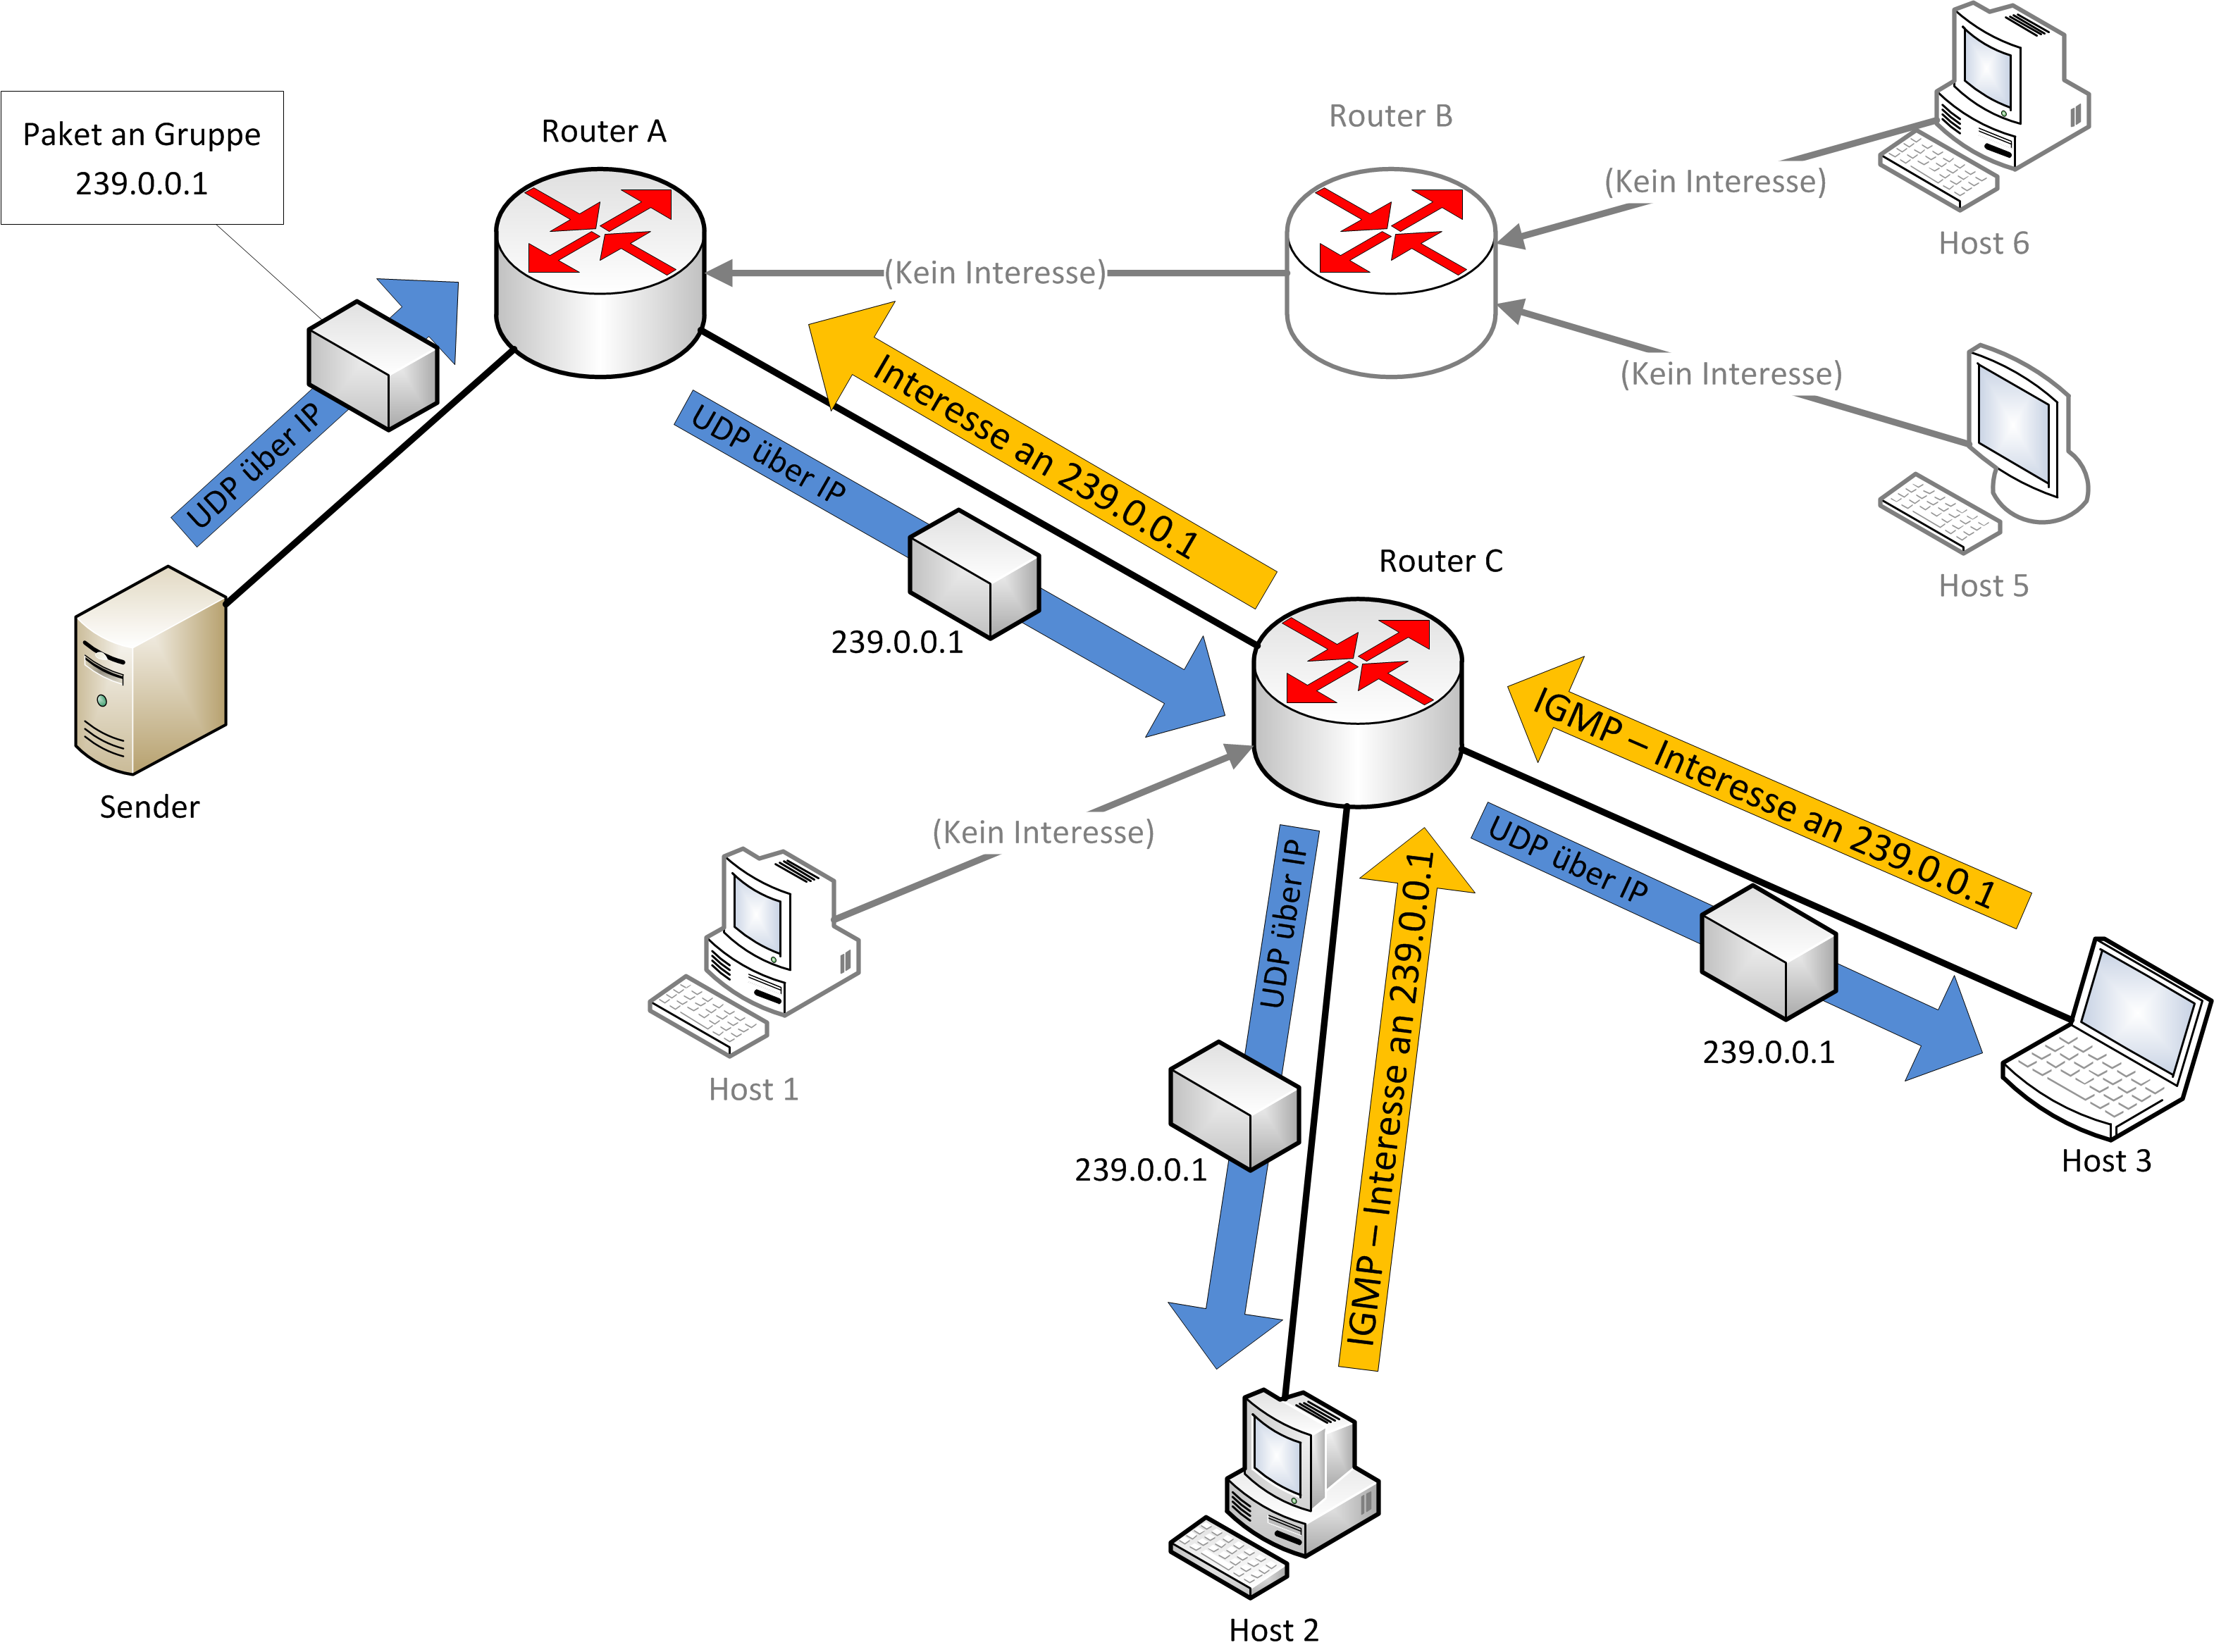
\includegraphics[width=15cm]{images/multicasting.png}
\centering
\caption{Schematische Verteilung eines Multicast-Pakets}
\label{mc_overview}
\end{figure}

Technisch wird Multicasting in OSI-Schicht 3 (Vermittlung/Network) bzw. der ihr
entsprechenden Internetschicht des TCP/IP-Referenzmodells umgesetzt.\\
\\
Wie oben erwähnt, wird Multicast-Datenverkehr durch Multicast-Gruppen und
dazugehörige IP-Adressen organisiert. Auf technischer Ebene heißt das, dass der
Sender in den IP-Header eines Datenpakets nicht die IP-Adresse eines bestimmten
Hosts, sondern eine Multicast-Adresse als Empfänger einträgt. Der
IP-Adressbereich von 224.0.0.0 bis 239.255.255.255 ist für
Multicast-Adressen reserviert (siehe hierfür z.B. RFC3171). Das so erzeugte
IP-Paket wird dann an den nächstgelegenen Router geschickt.\\
\\
Komplexe Multicast-Routing-Protokolle sorgen nun dafür, dass das Paket alle
Router, an die interessierte Hosts angeschlossen sind, erhalten. Um das Netzwerk
nicht unnötig zu belasten, sorgen sie auch dafür, dass Router, deren
angeschlossene Netzwerke überhaupt nicht am Multicast interessiert sind, die
Pakete auch nicht erhalten. Vor Allem muss aber vermieden werden, dass sich in
den Paket-Routen Zyklen bilden, da sie die Leistungsfähigkeit des Netzwerks
stark beeinträchtigen können. Auch wenn die Routing-Protokolle ebenfalls in
OSI-Schicht 3 agieren und \emph{Bestandteil} von IP sind, dienen sie selbst
\emph{nicht} der Datenübertragung. Sie dienen lediglich der Kommunikation der
Router untereinander, damit diese die Multicast-Pakete korrekt weiterleiten
können. Die Multicast-Pakete selber sind nach wie vor gewöhnliche IP-Pakete
(von der speziellen Empfängeradresse im Header abgesehen). Häufig verwendete
Multicast-Routing-Protokolle sind PIM, DVMRP (über IGMP, s.u.) und MOSPF.\\
\\
Um Multicast-Pakete zu empfangen, muss sich ein Host bei einer Multicast-Gruppe
anmelden. Er teilt dazu dem Router, an den er angeschlossen ist mit, dass er an
einer bestimmten Multicast-Gruppe interessiert ist. Die gewünschte
Multicast-Gruppe wird durch ihre Multicast-IP-Adresse spezifiziert. Der Router
weiß nun, dass der angeschlossene Host an allen Paketen interessiert ist, die
diese Multicast-Adresse im Empfängerfeld tragen. Der Host teilt dem Router sein
Interesse über das \emph{Internet Group Management Protocol (IGMP)} mit. Wie
die Routing-Protokolle ist auch dieses Protokoll wieder Teil von IP, dient aber
ebenfalls nicht der Datenübertragung selbst, sondern nur der Kommunikation der Netzwerkknoten
untereinander. Tatsächlich verwendet auch das oben erwähnte DVMRP zum
Informationsaustausch IGMP-Pakete.\\
\\
Das Versenden und Empfangen eines Multicast-Pakets, sowie die dazu
notwendige Interaktion der beteiligten Netzwerkkomponenten ist in Abbildung
\ref{mc_overview} schematisch dargestellt.

\section{Multicasting unter Java}

Die zum Einsatz kommende Java Platform Standard Edition 6 stellt für
Multicast-Anwendungen die \emph{MulticastSocket}-Klasse zur Verfügung. Der
MulticastSocket stellt Methoden zum transparenten Senden und Empfangen von
UDP-Multicast-Paketen bereit. Von der Anwendung werden zum Senden der
Paketinhalt und die Ziel-Gruppenadresse übergeben. Analog wird zum
Empfangen eines Multicast-Streams die gewünschte Gruppenadresse übergeben. Alle
übrigen zur Kommunikation benötigten Systemaufrufe und Mechanismen werden von
der Klasse verborgen. Eine gesonderte Auseinandersetzung mit IGMP oder
Multicast-Routing ist daher auf Anwendungsebene nicht mehr nötig. Aus Sicht des
OSI- und auch des TCP/IP-Schichtenmodells stellt ein Socket damit die Verbindung
zur Transportschicht (OSI-Layer 4) her.

\section{Einordung des Tools}

\begin{figure}[H]
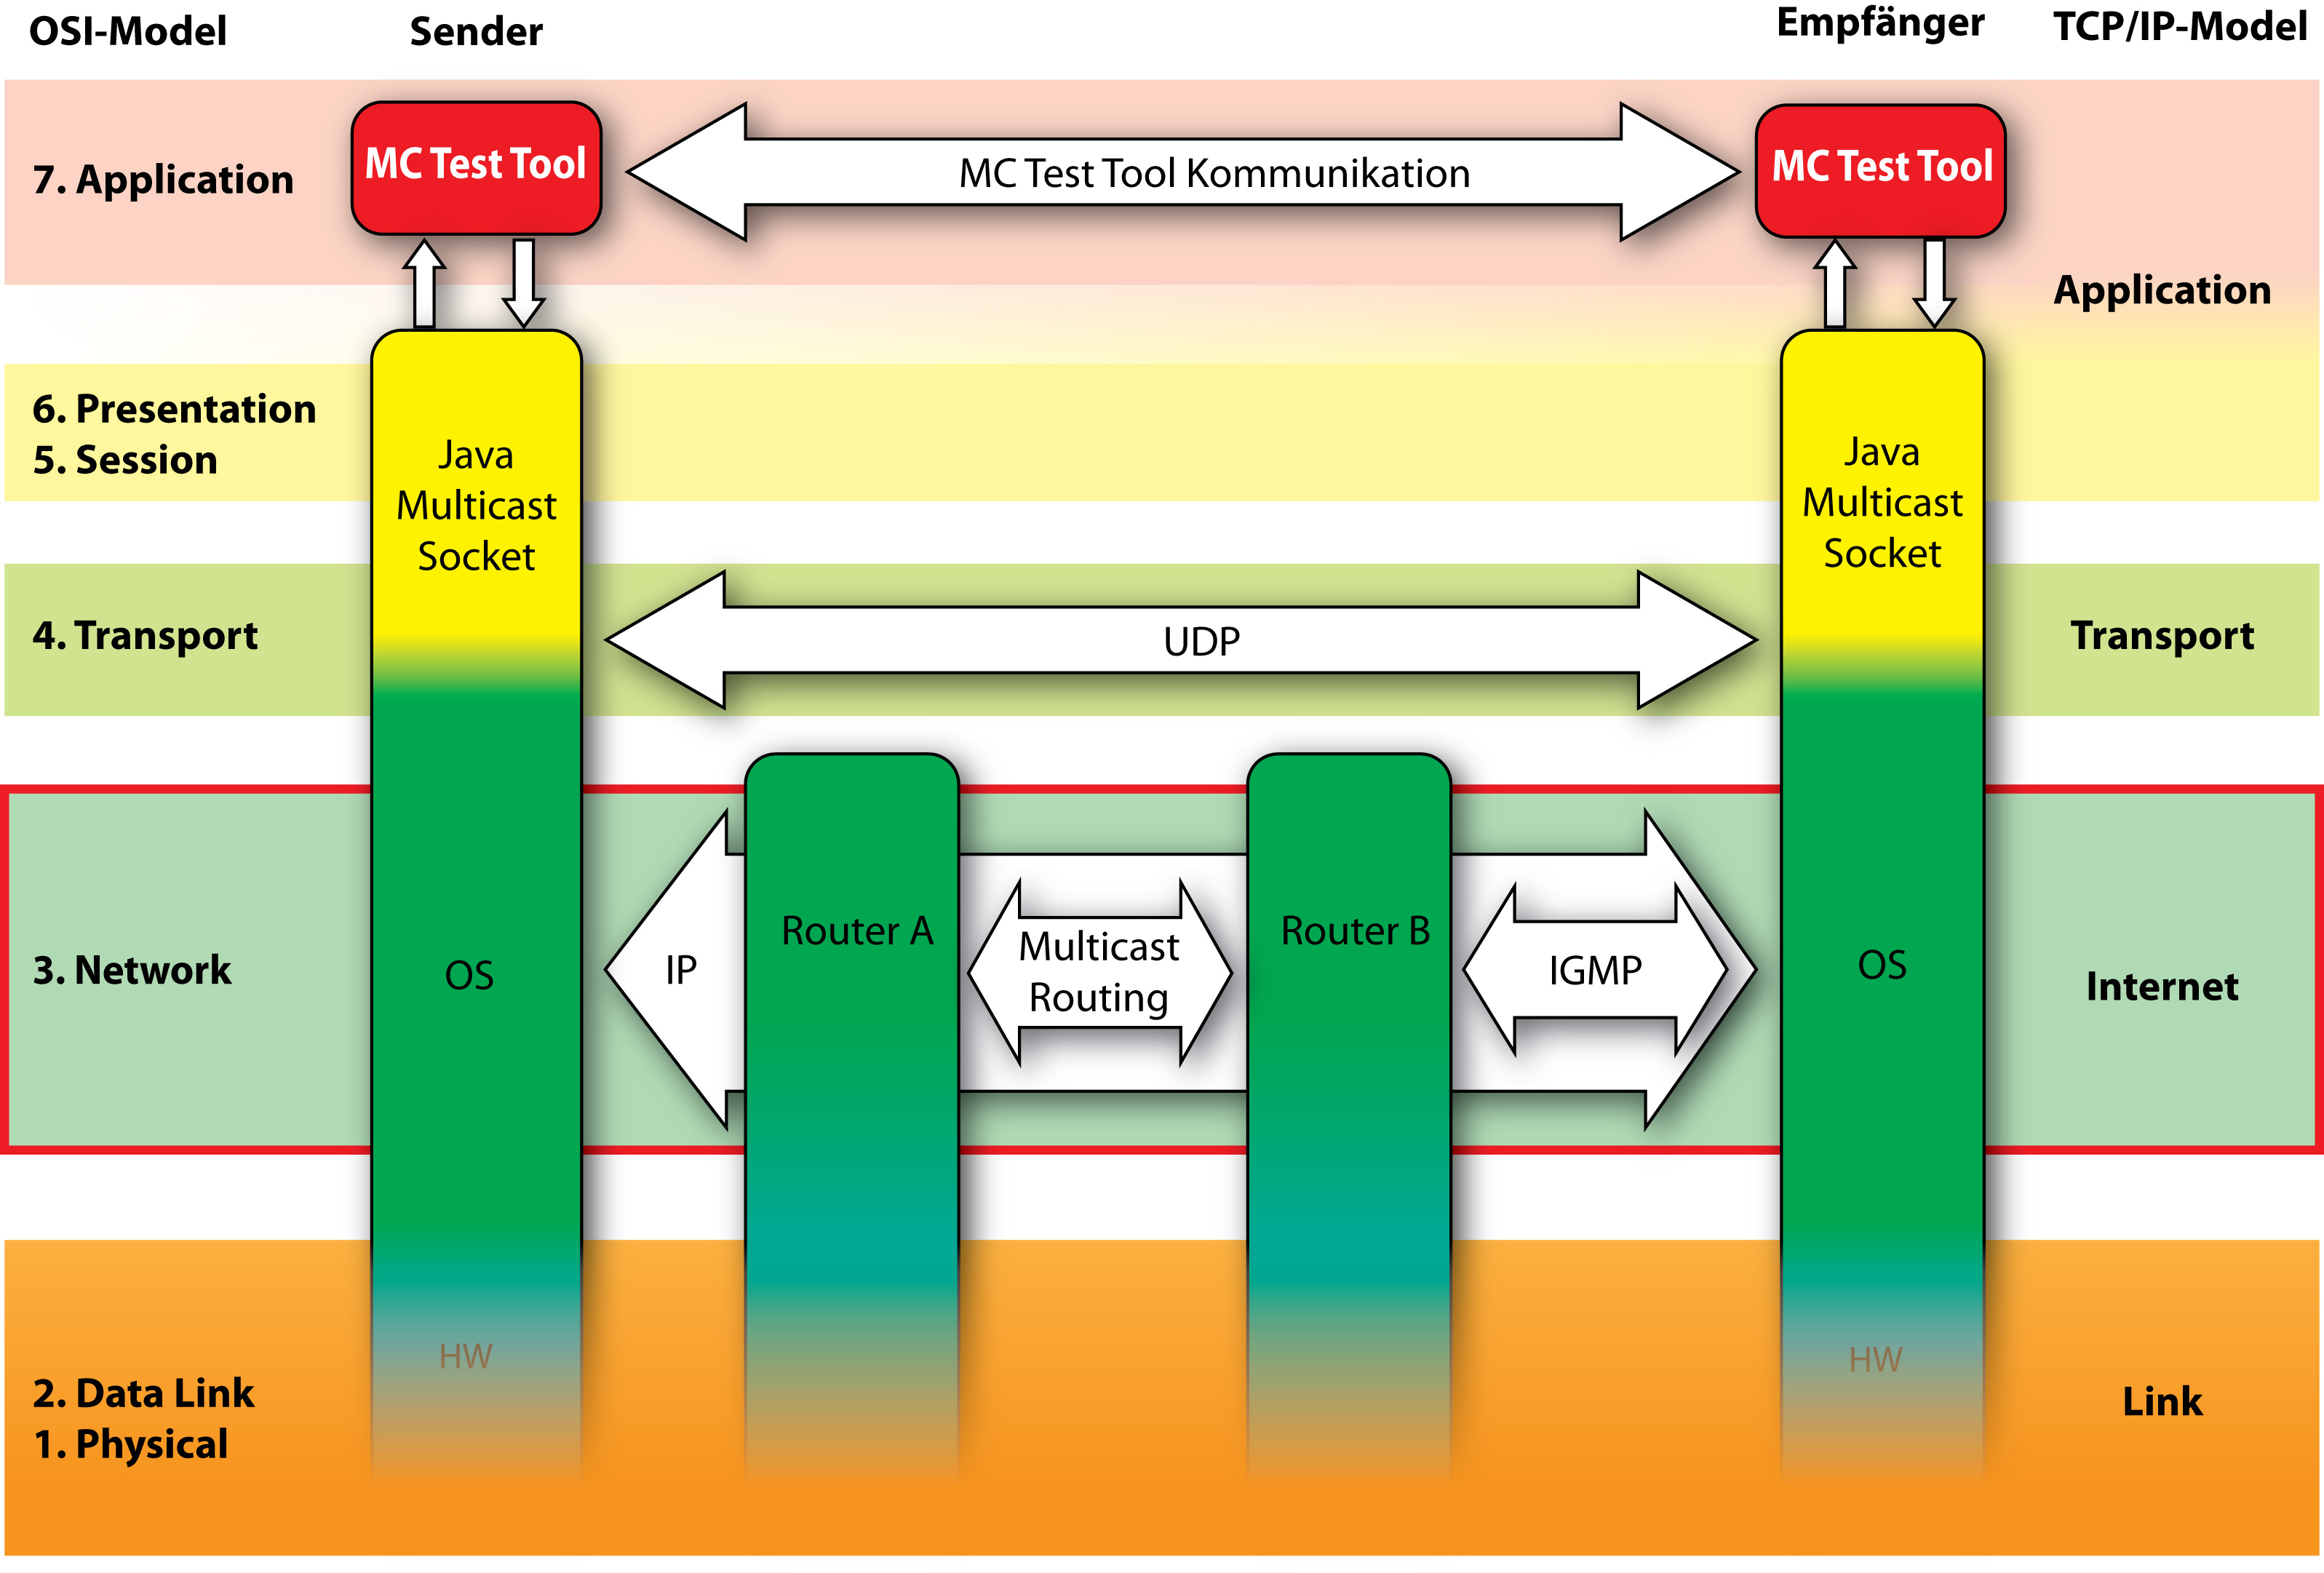
\includegraphics[width=15cm]{images/mc_osi_einordnung.jpg}
\centering
\caption{Einordnung des Gesamtsystems in das OSI- bzw. TCP/IP-Schichtenmodell}
\label{mc_osi_einordnung}
\end{figure}

Hauptaufgabe des Multicast Test Tools ist es, wie bereits beschrieben, die
Multicasting-Fähigkeiten eines Netzwerkes zu testen. Seine Analysen
konzentrieren sich also vor Allem auf die Netzwerkschicht (Schicht 3) des
OSI-Modells bzw. die Internetschicht des TCP/IP-Modells. Den Zugriff auf diese
Schicht stellt der MulticastSocket der Java Platform zur Verfügung. Obwohl also
die Netzwerkschicht Ziel der Untersuchungen ist, wird sich der tatsächliche
Programmieraufwand fast ausschließlich auf die Anwendungsschicht (OSI 7)
konzentrieren.\\
\\
Abbildung \ref{mc_osi_einordnung} gibt einen Überblick über die Einordnung des
Systems ins OSI- bzw. TCP/IP-Modell.
